\section{Моделювання результатів виконання тестових завдань}

\subsection{Інформаційний метод прогнозування часу розв’язання завдань}

Один з методів прогнозування часу розв’язання завдання людиною,
що використовується в інженерній психології, є інформаційний метод.
Вважаємо, що студент виконує завдання одне за одним.
Кожне завдання має певну складність $H_i$ --- кількість інформації,
що потрібно обробити для розв’язку завдання.
Студент виконує кожне завдання з певною швидкістю $V_i$.
Тоді час виконання тесту $\tau$ буде рахуватися за формулою
\begin{equation*}
  \tau = \sum_{i=1}^{l}\frac{H_i}{V_i},
\end{equation*}
де $l$ --- кількість задач. \cite{Lomov:1982}

Вважаємо, що швидкість виконання завдання $i$ рахується за формулою
\begin{equation*}
  V_i\left( t \right) = \frac{1}{\tau_i},
\end{equation*}
де $\tau_i$ --- випадкова величина, що має показниковий розподіл
з параметром $\lambda_i$, який залежить від типу вищої нервової діяльності
людини та часу, що затрачено на виконання попередніх завдань:
\begin{equation*}
  \tau_i \sim Exp\left( \lambda_i \right).
\end{equation*}
Тоді $\tau_i$ буде часом, що витрачається на одиницю інформації
завдання
\begin{equation*}
  \tau = \sum_{i=1}^{l} H_i \cdot \tau_i.
\end{equation*}
Якщо всі завдання мають однакову складність $H_i = H$, рівність приймає вигляд
\begin{equation*}
  \tau = H \cdot \sum_{i=1}^{l} \tau_i.
\end{equation*}

Щоб застосувати отримані з моделювання теппінг-тесту результаті,
потрібно горизонтально масштабувати параболи, до яких було аппроксимовано
ламані.
Початкова парабола $y$ має вигляд
\begin{equation*}
  y \left( t \right) = a^2 \cdot t + b \cdot t + c.
\end{equation*}
Потрібно отримати параболу $\lambda$
\begin{equation*}
  \lambda \left( t \right) = A^2 \cdot t + B \cdot t + C
\end{equation*}
таку, для якої виконується
\begin{equation*}
  \begin{split}
    \lambda\left( 0 \right) &= y\left( 0 \right), \\
    \lambda\left( T \right) &= y\left( t_t \right), \\
    \lambda\left( \frac{T}{2} \right) &= y \left( \frac{t_t}{2} \right)
  \end{split}
\end{equation*}
$t_t$ --- час виконання теппінг-тесту (30 секунд),
$T$ --- час виконання тестових завдань (40 або 90 хвилин).
Маємо розв’язок
\begin{equation*}
  \begin{split}
    A &= a \cdot \left( \frac{t_t}{T} \right)^2, \\
    B &= b \cdot \frac{t_t}{T}, \\
    C &= c,
  \end{split}
\end{equation*}
тобто
\begin{equation*}
  \lambda\left( t \right)
  = a \cdot \left( \frac{t_t}{T} \right)^2 \cdot t^2
    + b \cdot \frac{t_t}{T} \cdot t
    + c.
\end{equation*}

Отже маємо
\begin{equation*}
  \begin{split}
    \tau_1 &\sim Exp\left\{ \lambda\left( 0 \right) \right\}, \\
    \tau_i &\sim
      Exp\left\{ \lambda\left( \sum_{j=1}^{i} H_j \cdot \tau_j \right) \right\},
      \qquad i>1.
  \end{split}
\end{equation*}

\subsection{Моделювання тесту}

Було змодельовано тестування на півтори години з $10$ задачами,
кожна з яких має складність $H=0.5$.
Номер задачі, яку виконує студент на даний момент, фиксується кожні $10$
секунд.
Для застосування методу головних компонент
було змодельовано проходження тестування $600$ студентами.

На рис. \ref{fig:pca:main} можна побачити дисперсії перших десяти головних
компонент.
Майже половину інформації ($44.6\%$) можна отримати з першої компоненти.
\begin{figure}[h]
  \centering
    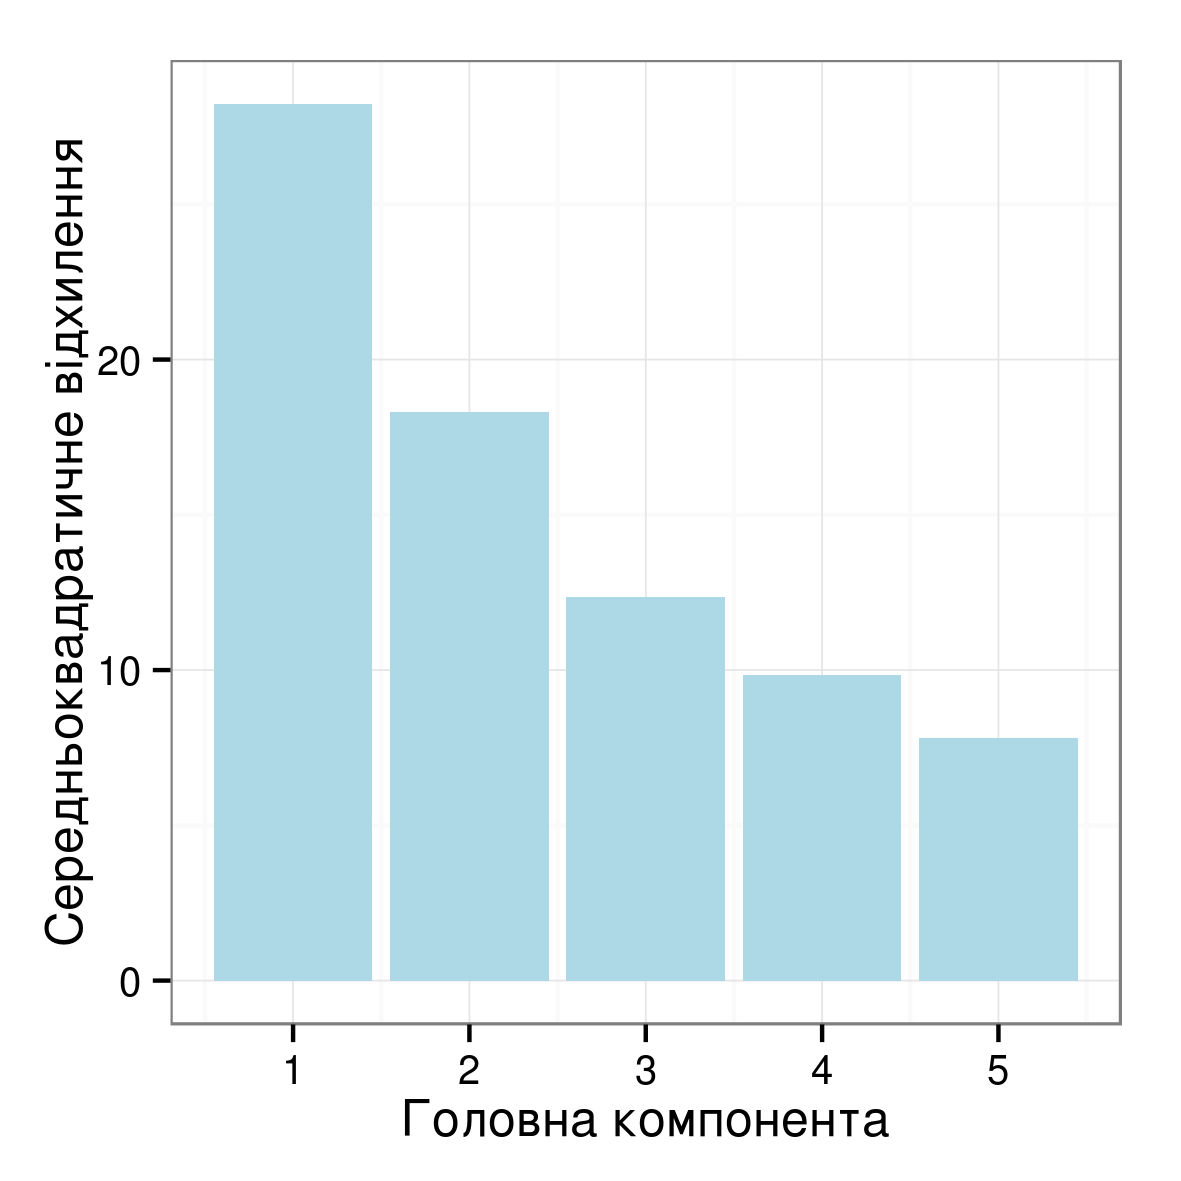
\includegraphics{images/pca}
  \caption{Дисперсії першого десятку головних компонент}
  \label{fig:pca:main}
\end{figure}
На рис. \ref{fig:pca:histograms} наведено гістограми перших чотирьох
головних компонент.
\begin{figure}[h]
  \centering
    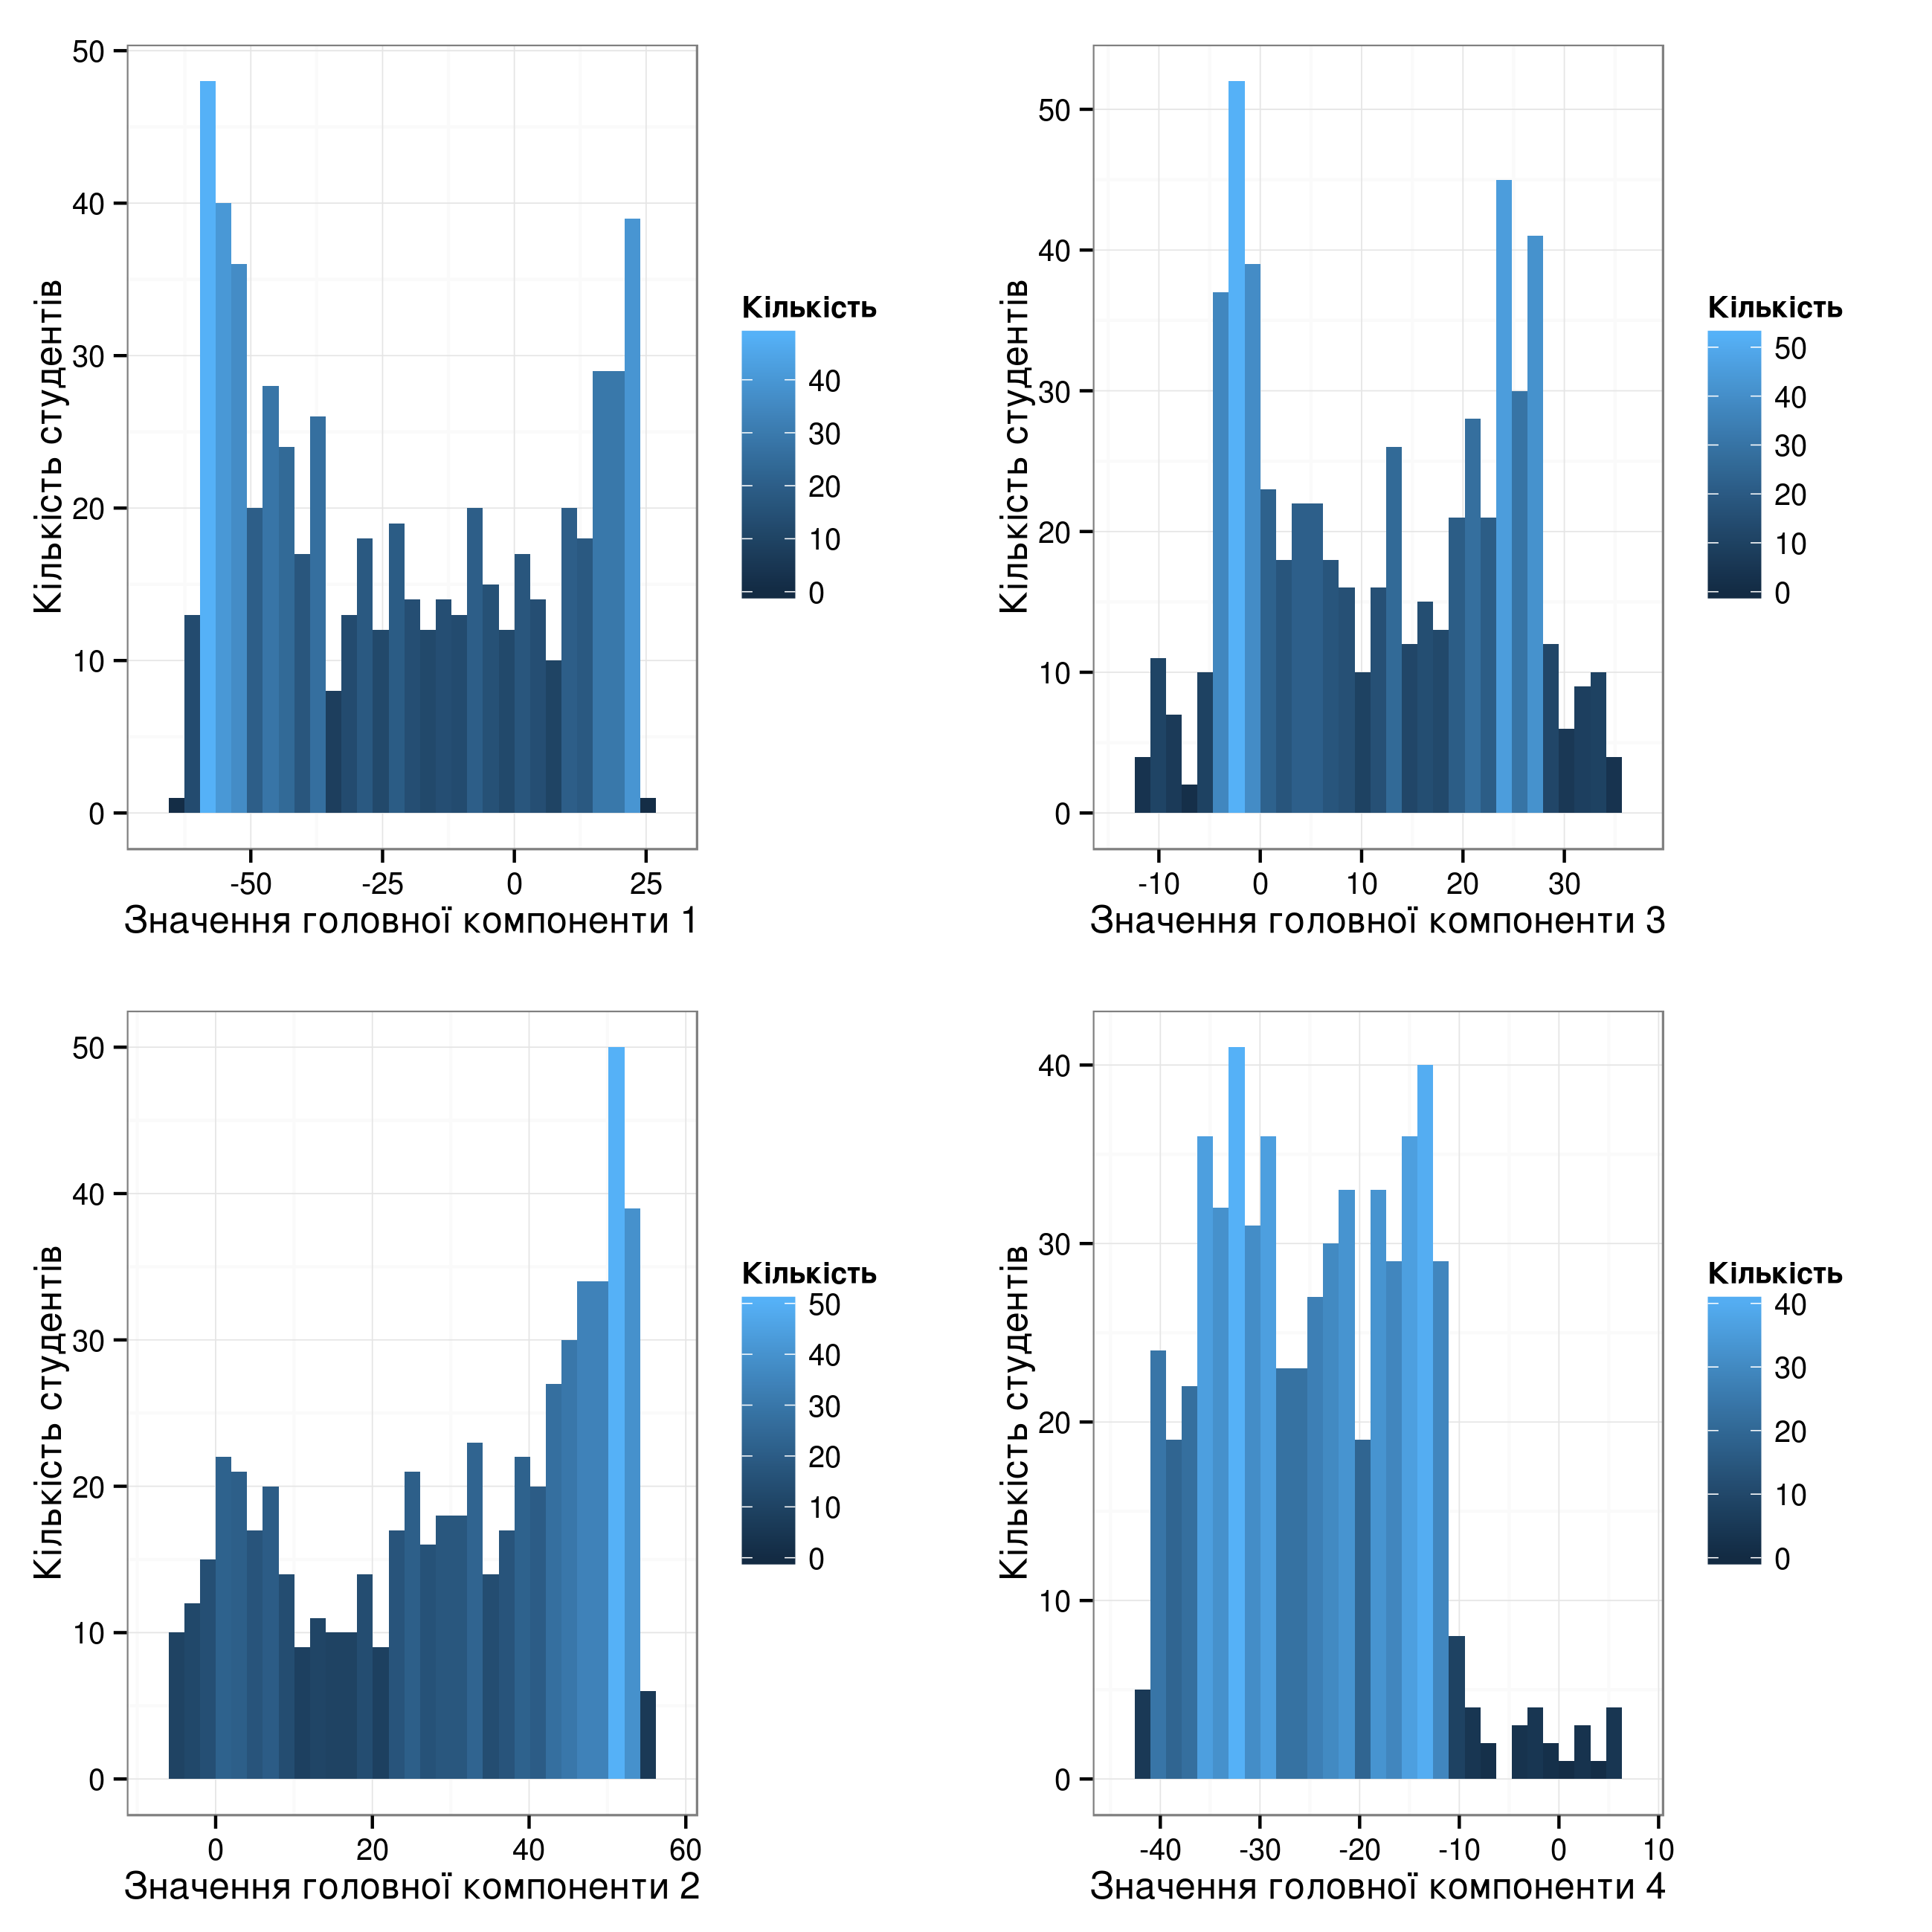
\includegraphics[width=\textwidth]{images/pca_hists}
  \caption{Гістограми першої четвірки головних компонент}
  \label{fig:pca:histograms}
\end{figure}
Але з рис. \ref{fig:pca:histograms:detailed} видно, що доцільно
використовувати лише першу компоненту, а також не вдасться відрізнити
від інших класів змішаний та неврівноважений тип.
\begin{figure}[h]
  \centering
    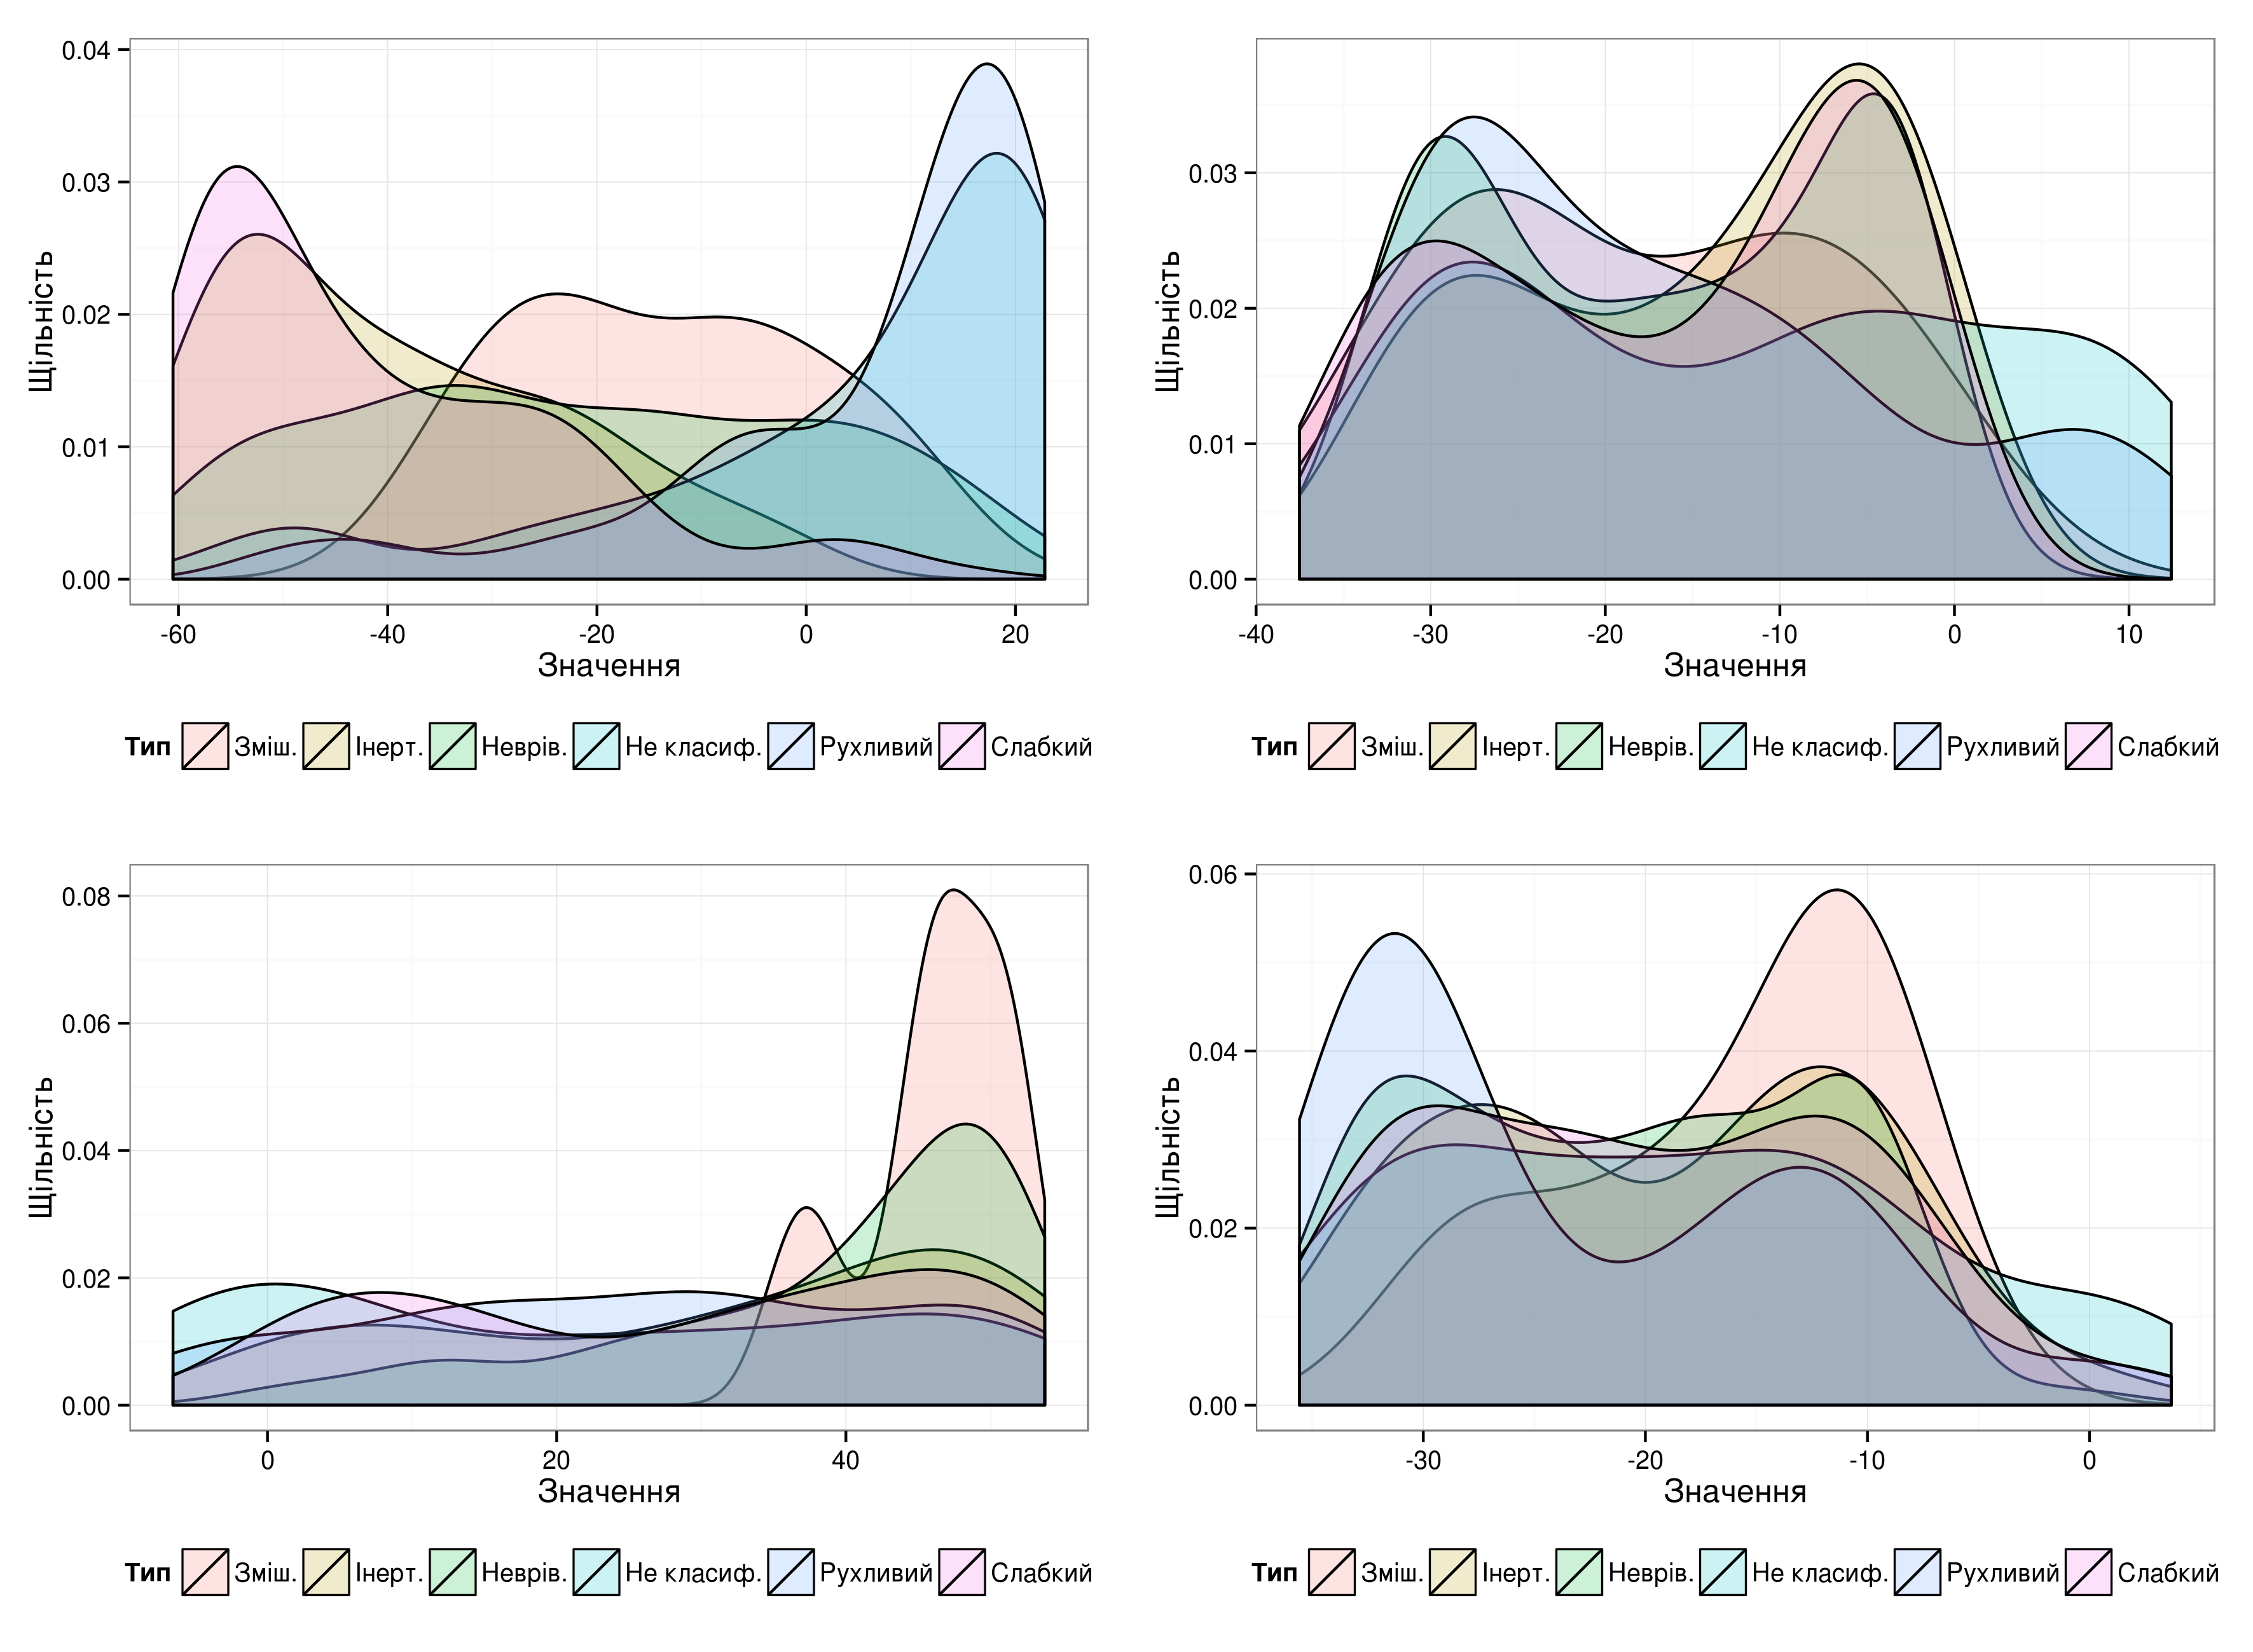
\includegraphics[width=\textwidth]{images/pca_hists_detailed}
  \caption{Детализовані гістограми першої четвірки головних компонент}
  \label{fig:pca:histograms:detailed}
\end{figure}
На рис. \ref{fig:pca1} зображено склад першої головної компоненти
з усіма класами та без змішаного і неврівноваженого типів.
\begin{figure}[h]
  \centering
    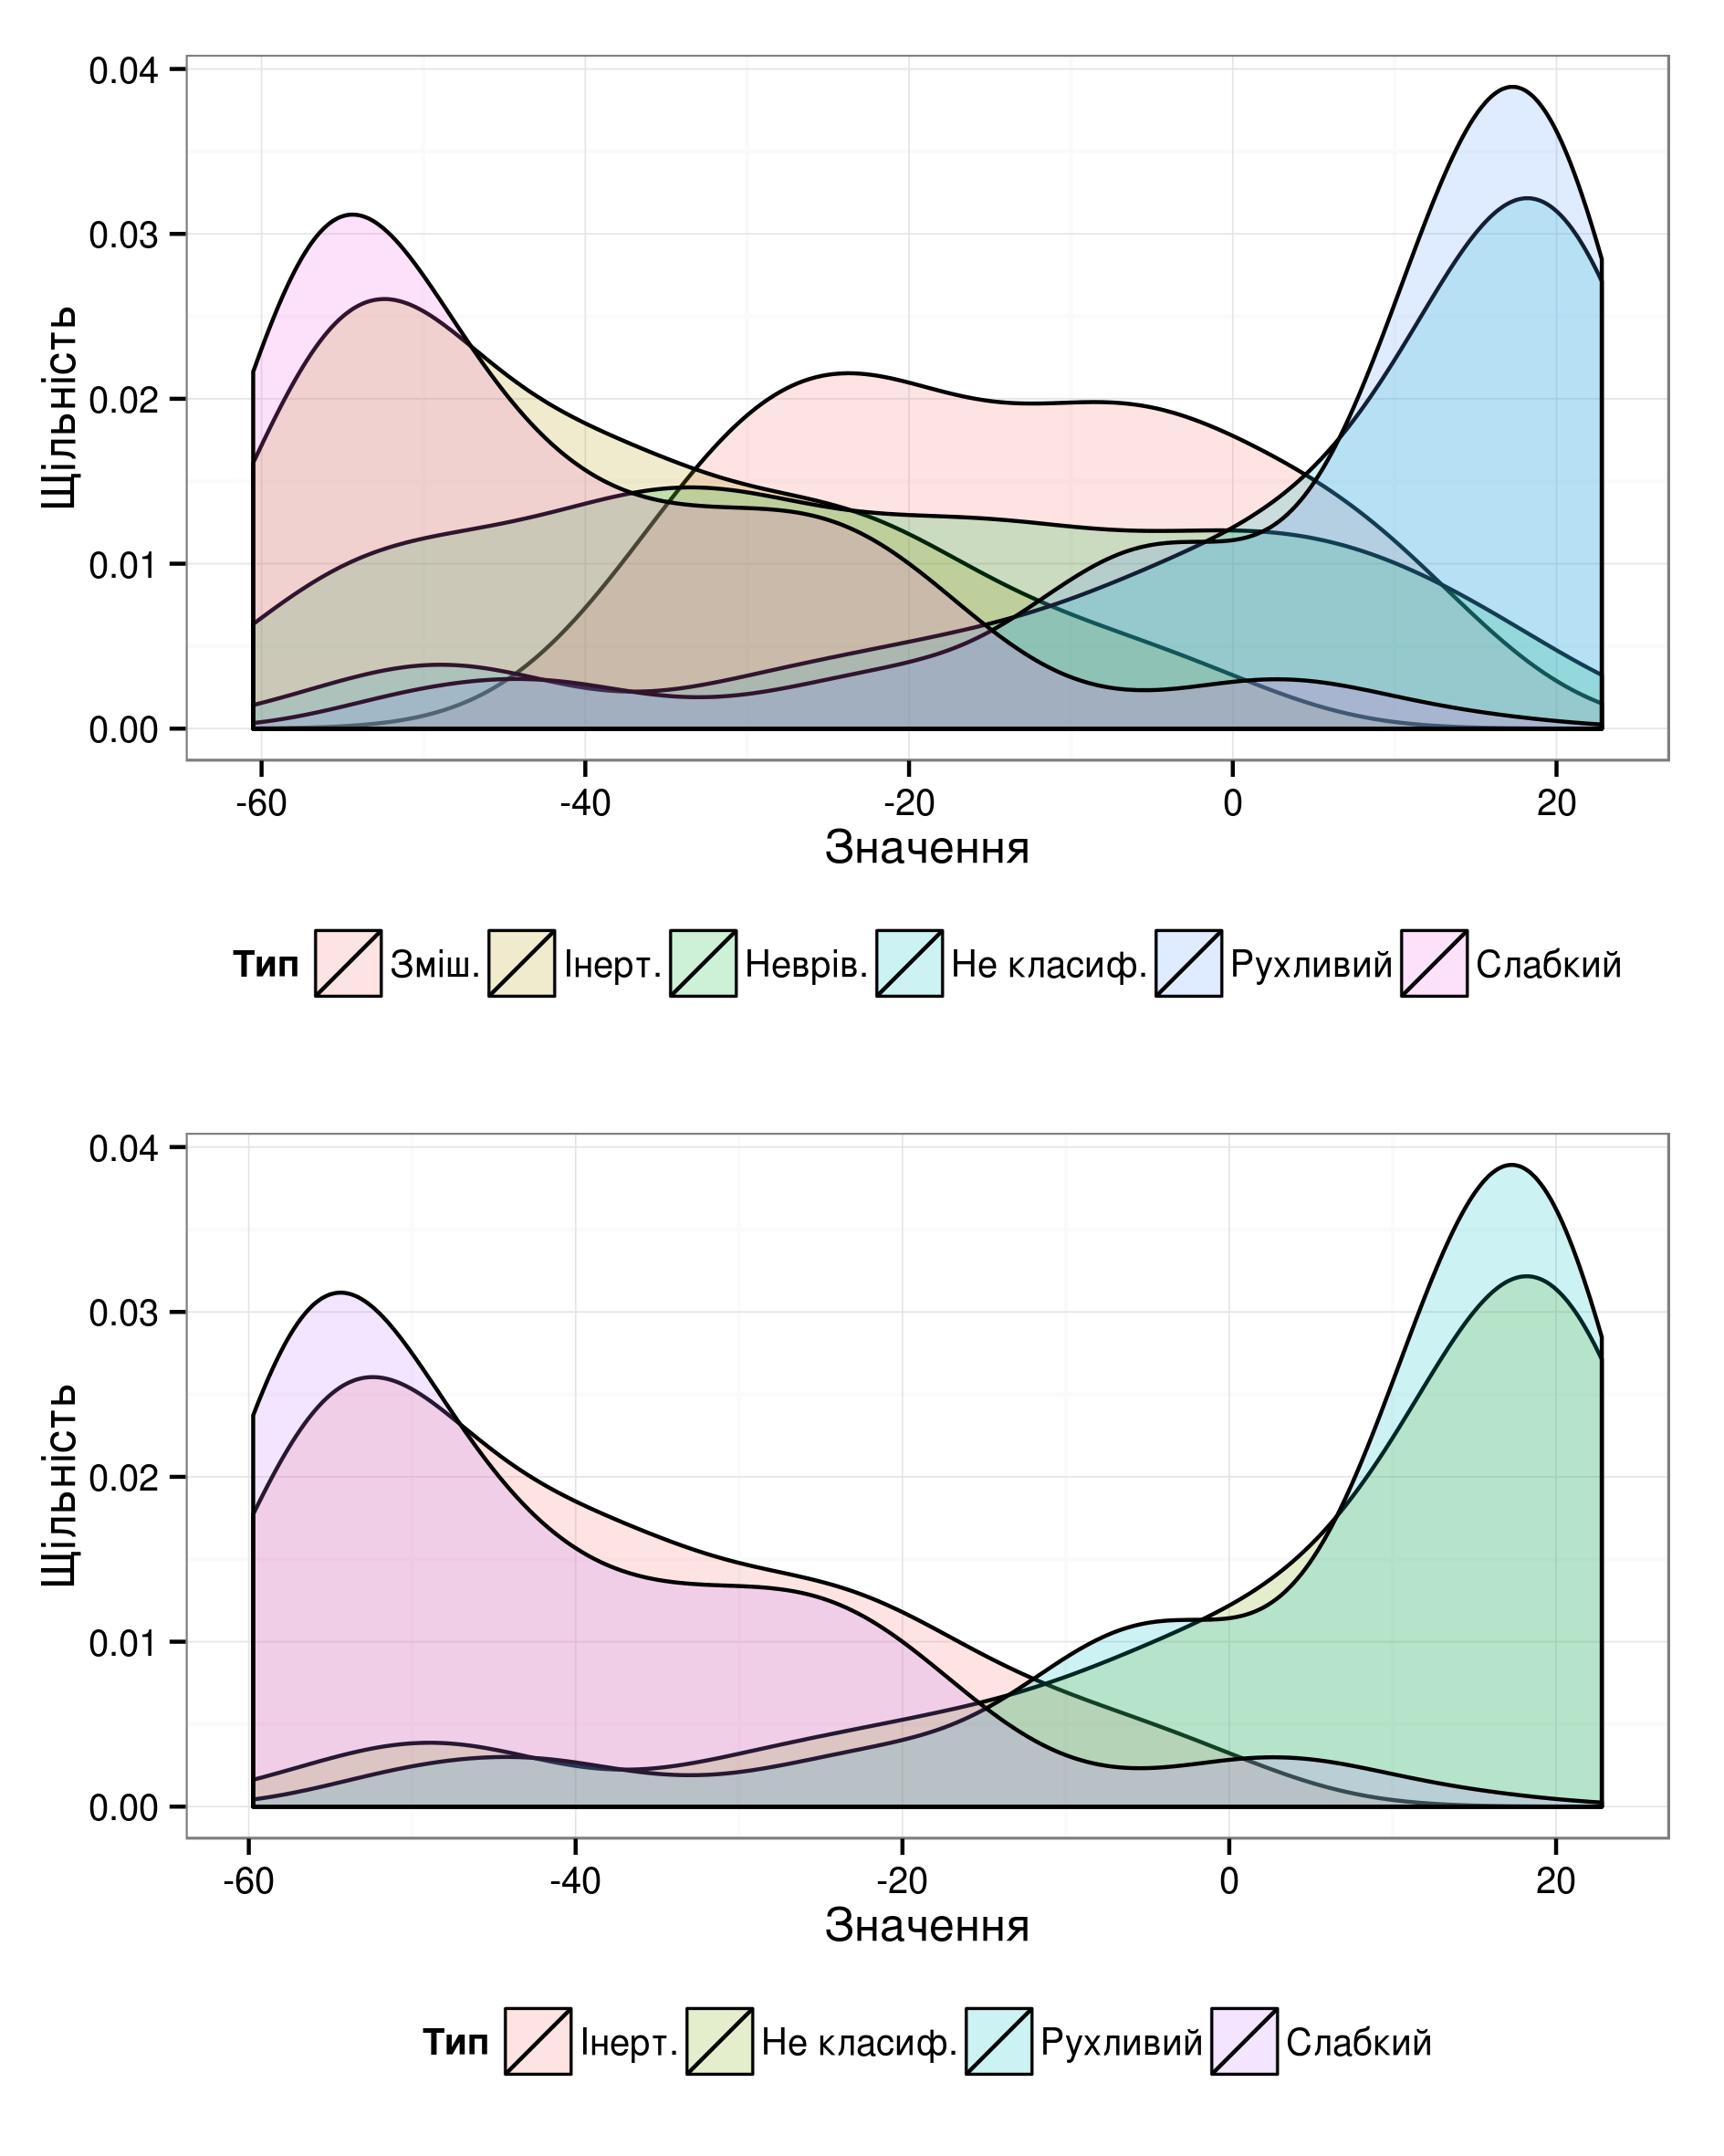
\includegraphics[width=\textwidth]{images/pca1_hist}
  \caption{Детализовані гістограми першої головної компоненти}
  \label{fig:pca1}
\end{figure}
За допомогою алгоритму CART (Classification and Regression Tree) було
класифіковано дві групи студентів:
\begin{enumerate}
  \item
    Ті, кому треба більше часу думати і не поспішати при виконанні завдань,
    щоб запобігти помилок --- рухливий клас, а також не класифіковані
    студенти, адже в основному не вдалося віднести до того чи іншого типу
    тих студентів, активність яких не спадає з часом.
  \item
    Ті, кому треба більше уваги приділяти елементарним задачам,
    щоб довести до автоматизму їх розв’язання і не витрачати час на
    зайві дії --- це студенти, що відносяться до слабкого та інертного типу.
\end{enumerate}
Дерево класифікації зображено на рис. \ref{fig:tree:simple}.
Як можна побачити, критерій досить простий:
\begin{itemize}
  \item
    ті студенти, перший головний крітерій яких перевищує поріг $17.155$,
    відносяться з ймовірністю біля $90\%$ до тих, яким треба більше
    тренуватися;
  \item
    ті студенти, перший головний крітерій яких не перевищує поріг $17.155$,
    відносяться з ймовірністю біля $90\%$ до тих, яким треба більше думати.
\end{itemize}
\begin{figure}[h]
  \centering
    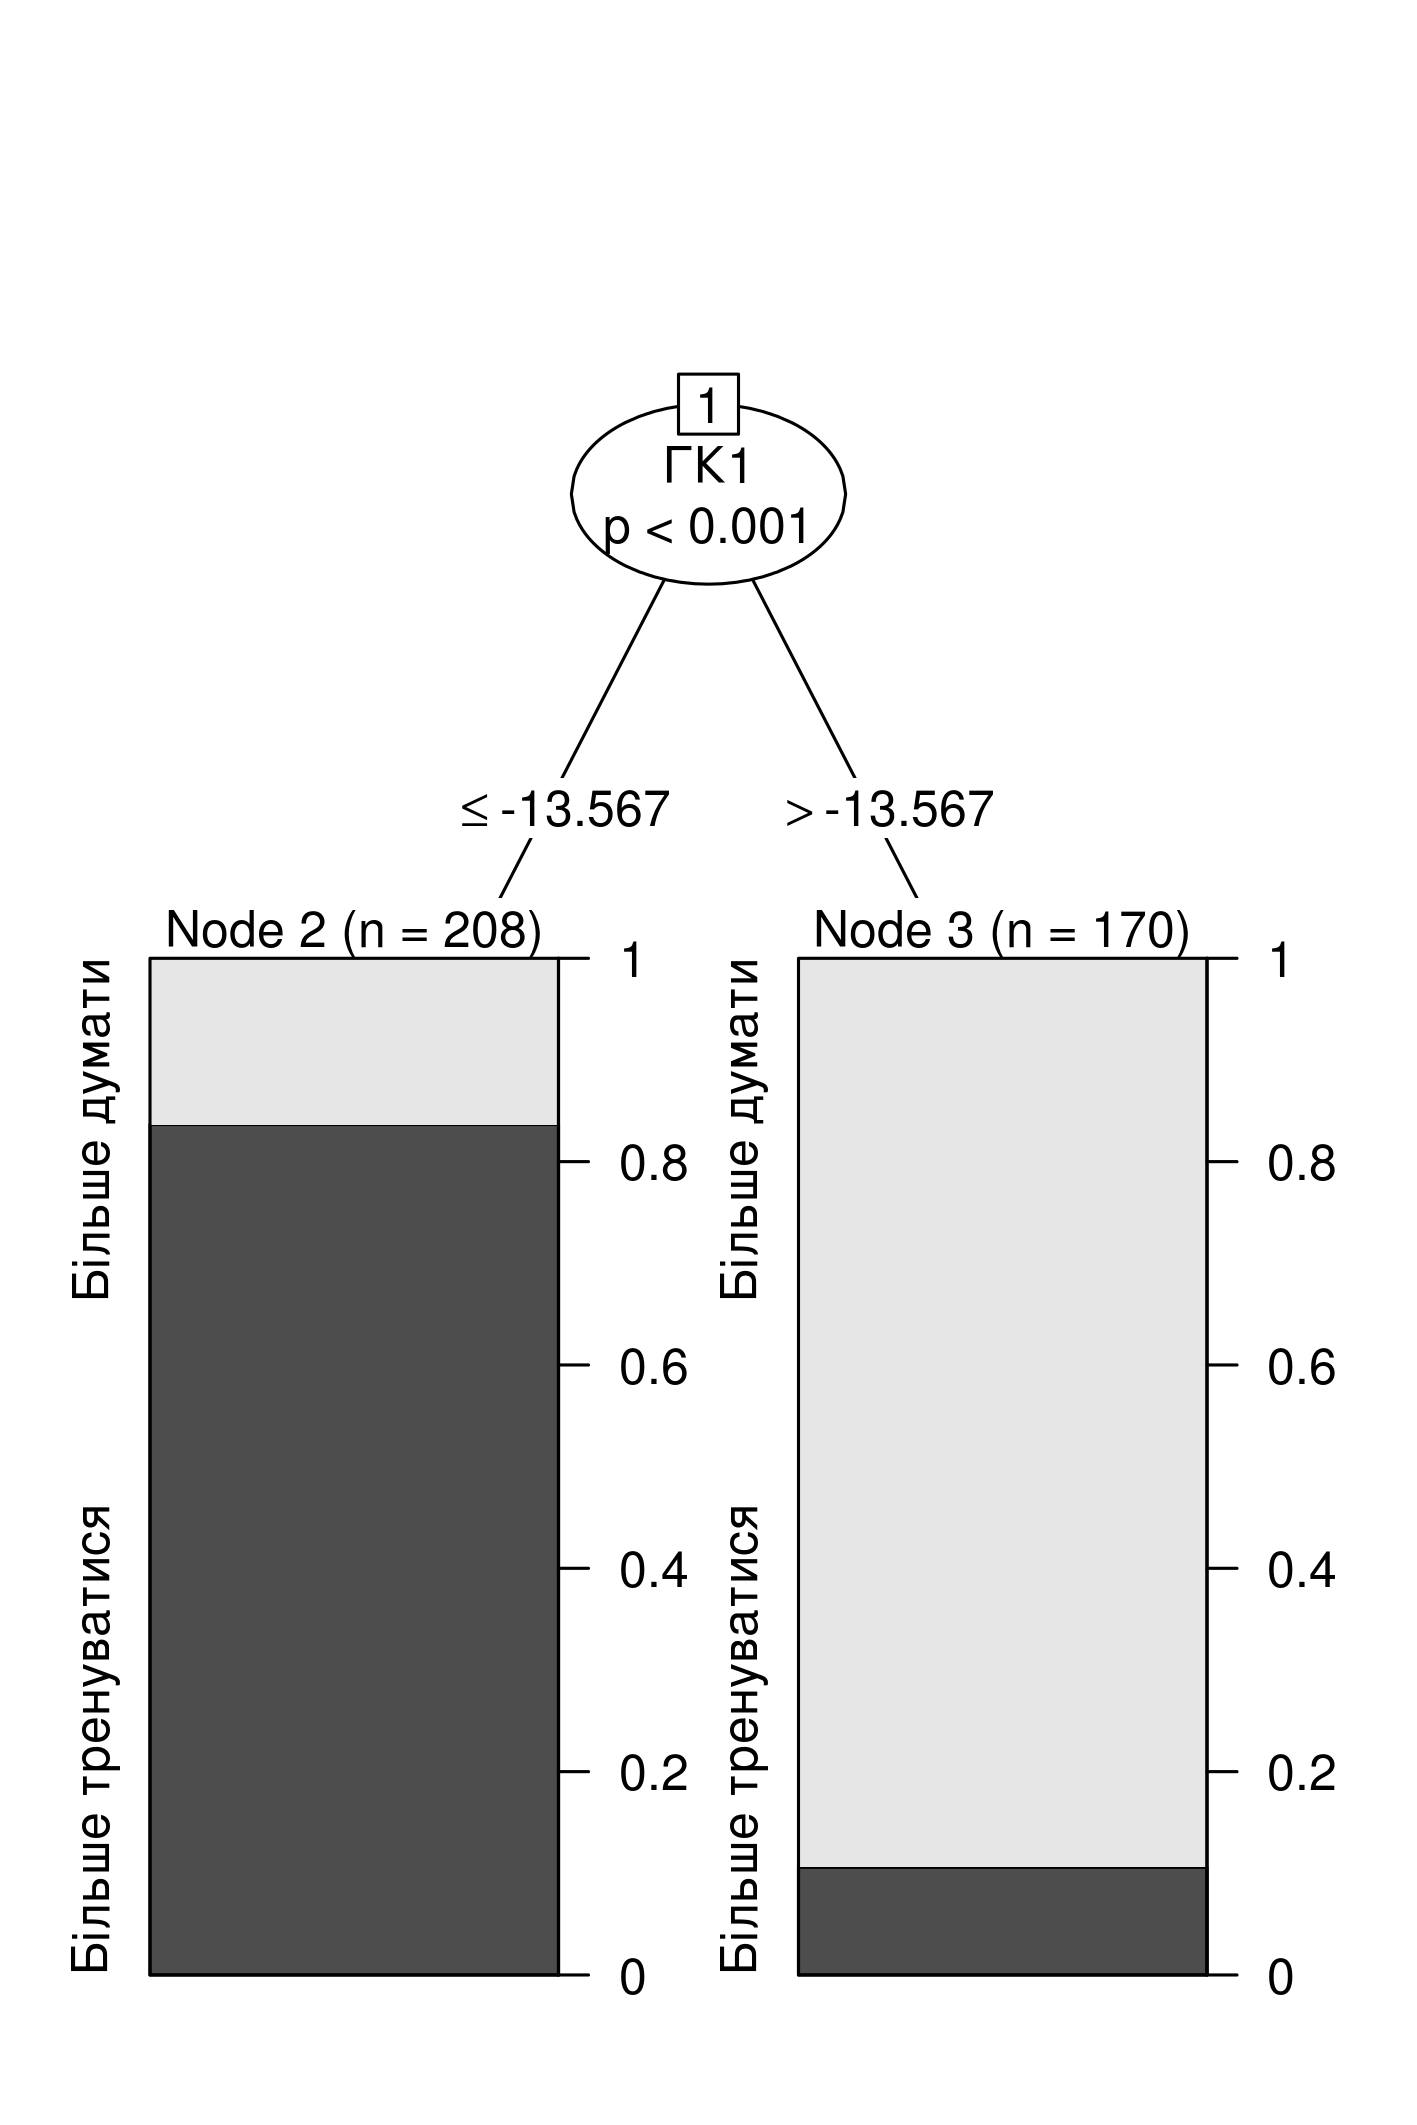
\includegraphics{images/tree}
  \caption{Дерево класифікації}
  \label{fig:tree:simple}
\end{figure}
